\subsection{Введение}
Многие химические и физические сигналы регулируют обработку генетической информации в живых клетках.
У эукариот эта регуляция в основном происходит на уровне нуклеосом - последовательных отрезков ДНК, обернутых вокруг октамеров гистоновых белков \cite{kornberg_chromatin_1974,olins_spheroid_1974}. Четыре типа гистонов (H3, H4, H2A, H2B) образуют два типа димеров (H3-H4, H2A-H2B). Четыре димера образуют октамер с двойной осью симметрии (диадной осью) \cite{burlingame_crystallographic_1985}. Как известно из кристаллографических исследований, примерно 147 пар оснований ДНК резко изгибаются вокруг октамера в $\sim$1,7 витка левой суперспирали, формируя коровую частицу нуклеосомы (NCP) \cite{luger_crystal_1997} (Рис. \ref{fig:p2_3:f1}а).

При формировании нуклеосом жесткая макромолекула ДНК с персистентной длиной около 50 нм должна резко изгибаться до радиуса кривизны всего в 5 нм. Это возможно благодаря электростатическому взаимодействию отрицательно заряженной ДНК с положительно заряженными гистонами, дополненному индивидуализированным паттерном взаимодействия белок-ДНК на атомном уровне в 14 сайтах связывания ДНК (по 7 с каждой стороны NCP). Эти сайты связывания расположены в положениях, где малая бороздка ДНК обращена к поверхности октамера и обычно присутствует боковую цепь остатка аргинина, которая выступает в пространство малой бороздки. Общая энергия взаимодействий гистонов с ДНК в нуклеосомах оценивается как не менее 23 ккал/моль \cite{onufriev_nucleosome:_2019}.
Стабильность нуклеосом может варьироваться на 2-4 ккал/моль в зависимости от гибкости последовательности ДНК \cite{thastrom_sequence_1999}, которая, как было показано, зависит от содержания GC, наличия гибких динуклеотидных ступеней YR, участков поли (dA:dT), эпигенетических модификации оснований ДНК, таких как 5-метилцитозин и т. д. \cite{ngo_asymmetric_2015,chua_mechanics_2012,zhurkin_sequence-dependent_1985,segal_genomic_2006}. Еще одним важным фактором являются вариации последовательности гистонов. Несмотря на то, что гистоновые белки одни из самых консервативных белков в эволюционном смысле, они подвержены множеству функционально значимых вариаций, включая посттрансляционные модификации (ПТМ) \cite{zhao_comprehensive_2015} и изменение последовательности за счет включения вариантов, изоформ и мутаций гистонов \cite{draizen_histonedb_2016,singh_replication-dependent_2018,nacev_expanding_2019}.

Представление о нуклеосомах как о средстве простой компактизации ДНК теперь устарело.
% Благодаря своей роли в обеспечении доступа к ДНК, нуклеосомы играют ключевую роль в эпигенетической регуляции экспрессии генов.
Различные режимы АТФ-зависимой и АТФ-независимой динамики нуклеосом, модулируемые гистоновым составом и последовательностью ДНК, обеспечивают богатый динамический ландшафт для регуляции генома \cite{armeev_linking_2019}. Например, скольжение нуклеосом с помощью АТФ-зависимых ремоделеров хроматина \cite{paul_regulation_2018} или их реконфигурация с помощью РНК-полимераз \cite{kujirai_transcription_2020,gaykalova_structural_2015} в значительной степени вовлечены в транскрипцию и ее регуляцию. Пассивная динамика нуклеосом также участвует во многих процессах. Новаторские эксперименты Джона Видома показали, что временное отворачивание ДНК от октамера гистонов может быть использовано факторами транскрипции для доступа к их сайтам связывания \cite{li_rapid_2005}. Недавние исследования методами FRET \cite{gansen_high_2018,sabantsev_direct_2019}, ЯМР \cite{sinha_distortion_2017, kitevski-leblanc_investigating_2018}, крио-ЭМ \cite{li_mechanism_2019,bilokapic_structural_2018} и масс-спектрометрии\cite{hada_histone_2019,sanulli_hp1_2019,sinha_distortion_2017} свидетельствуют о том, что существуют более тонкие режимы конформационной динамики нуклеосом, которые воспринимаются и используются белками хроматина. Например, кручение ДНК внутри NCP обеспечивает путь для АТФ-зависимого ремоделирования нуклеосом \cite{bowman_remodeling_2019,li_mechanism_2019}. Внутренняя динамика (пластичность) гистонового ядра также участвует в этом процессе (хотя на этот счет и ведутся дискуссии) \cite{sinha_distortion_2017,yan_structures_2019,armache_cryo-em_2019}. Сообщалось, что подавление этой динамики путем введения сайт-специфичных дисульфидных сшивок в отдельные димеры H3-H4 ингибирует передвижение нуклеосом ремоделером SNF2h, увеличивает вытеснение октамера комплексом RSC \cite{sinha_distortion_2017}, блокирует термически индуцированную диффузию нуклеосом вдоль ДНК \cite{bilokapic_structural_2018} и даже нарушает компактизацию хроматина белком HP1 \cite{sanulli_hp1_2019}. Эти результаты свидетельствуют о том, что октамер гистонов может принимать конформации, альтернативные тем, которые наблюдаются в рентгеновских структурах. Действительно, используя передовые методы крио-ЭМ, Bilokapic et al. недавно наблюдали некоторые альтернативные конформации нуклеосом с развернутой ДНК, наклоненными гистоновыми $\alpha$-спиралями и общей сжатой формой NCP \cite{bilokapic_structural_2018,bilokapic_histone_2018}. Еще большие внутренние флуктуации в структуре октамера гистонов предполагают эксперименты по химической сшивке лизинов \cite{hada_histone_2019} и эксперименты FRET с высоким разрешением\cite{gansen_high_2018}.


Эти и другие исследования подчеркнули существование нового уровня динамической сложности нуклеосом, связанного с атомистическими деталями структуры. Однако структурная интерпретация этих результатов все еще остается не вполне ясной. \textit{In silico} подходы, такие как моделирование методом молекулярной динамики (МД), являются мощными инструментами, которые могут дополнять экспериментальные методы и помочь механистически интерпретировать экспериментальные результаты с высоким уровнем детализации. До сих пор моделирование с помощью МД применялось для изучения распределения ионов вокруг нуклеосом и их гидратации \cite{materese_counterion_2009}, деталей разворачивания ДНК, скольжения и разборки нуклеосом \cite{ettig_dissecting_2011, rychkov_partially_2017, zhang_exploring_2016, winogradoff_molecular_2019,brandani_dna_2018,lequieu_silico_2017}, динамики гистоновых хвостов\cite{erler_role_2014, shaytan_coupling_2016,chakraborty_molecular_2018,morrison_conformation_2018}, эффектов посттрансляционных модификаций гистонов \cite{fenley_modulation_2018,li_investigating_2018,rajagopalan_structural_2017} и их вариантов \cite{bowerman_unique_2019}, эффектов влияния последовательности ДНК \cite{sun_tmb_2019} на динамику нуклеосом, взаимодействия между олигонуклеосомами \cite{collepardo-guevara_chromatin_2015} и гистоном H1 \cite{ozturk_chromatosome_2020,perisic_sensitive_2019} и т. д. Из-за вычислительной сложности такого рода расчетов часто прибегают к упрощениям (например, удаляют гистоновые хвосты, используют неявные модели растворителя или крупно-зернистое представление молекулярной системы), либо ограничивают временные рамки моделирования. В настоящее время наиболее известные МД исследования нуклеосом в полноатомном приближении были ограничены несколькими микросекундами времени моделирования \cite{winogradoff_molecular_2019,chakraborty_molecular_2018} даже с применением специализированных суперкомпьютеров, таких как ANTON. Однако предполагается, что важные функциональные переходы в структуре нуклеосом происходят в масштабе времени от микросекунды до миллисекунды \cite{gansen_high_2018}. Новые режимы функциональной динамики в этих временных масштабах все еще ждут подробных структурных исследований с помощью МД-моделирования.

В работе данного раздела, мотивированные различными новыми экспериментальными доказательствами ранее неизвестных способов конформационной динамики и пластичности нуклеосом, мы систематически исследовали равновесную динамику нуклеосом с помощью полноатомного МД-моделирования на масштабе времени 10 микросекунд и более.
Насколько нам известно, это первый случай, когда такие длинные динамические траектории анализируются для максимально реалистичных атомистических моделей NCP с полноразмерными гистоновыми хвостами при физиологической температуре и ионной силе. С помощью специально разработанных алгоритмов анализа траекторий (проекция координат в системе отсчета нуклеосом, расчет относительного скручивания ДНК, анализ стабильных контактов и т. д.) мы выявили новые режимы динамики и пластичности нуклеосом. Мы наблюдаем реконфигурацию и разворачивание концов ДНК в нуклеосомах, опосредованных гистоновыми хвостами H3 и H2A, образование дефектов кручения в ДНК и сдвиг ориентационного положения для части коровой ДНК, структурную пластичность ядра гистона в соответствии с недавними экспериментальными наблюдениями. В данном разделе также обсуждается значение наших результатов для понимания ремоделирования нуклеосом и организации структуры хроматина более высокого порядка.


\subsection{Материалы и методы}
\subsubsection{Молекулярно-динамические расчеты}
Моделирование проводилось с использованием пакета GROMACS 2018.1 с поддержкой графических ускорителей \cite{abraham_gromacs:_2015} с силовым полем Amber ff14SB \cite{maier_ff14sb_2015}, дополненным поправками parmbsc1 \cite{ivani_parmbsc1_2016} для ДНК и поправками ионных параметров CUFIX \cite{yoo_new_2018}. Начальные координаты были получены из соответствующих структурных файлов в базе данных PDB (см. таблицу \ref{tbl:p2_3:systems}). Для моделирования системы NCP$_{147}$ конформация хвостов гистонов для одной половины NCP (цепи E, F, G, H) была скорректирована, чтобы соответствовать конформации симметричных цепей на другой половине NCP (цепи A, B, C, D). Для моделирования с усеченными гистоновыми хвостами хвосты усекались согласно позициям, изображенным на рисунке \ref{fig:p2_3:f1}д. Сайты усечения были выбраны таким образом, чтобы удалить гибкие части хвостов гистонов, при этом оставляя некоторые части близкие к глобулярному ядру, которые устанавливают стабильные контакты с ДНК или гистонами (например, N-хвосты H3 и H2B, выступающие между супервитками ДНК или H2A C-хвост, взаимодействующий с димером H3-H4). Для моделирования с фиксированными гистоновыми фолдами, C $\alpha$-атомы спиралей $\alpha1$, $\alpha2$ и $\alpha3$ во всех гистонах удерживались в их исходных положениях с использованием гармонического потенциала с силовой постоянной 1000 кДж/моль/нм$^2$. Все системы были помещены в ячейку для моделирования в виде усеченного октаэдра с периодическими граничными условиями, установленными на расстоянии не менее 2 нм от атомов NCP. Следующим шагом в ячейку добавлялись молекулы воды модели TIP3P \cite{jorgensen_comparison_1983} для сольватации NCP, затем были добавлены ионы Na и Cl, чтобы нейтрализовать заряд и довести ионную силу до 150 мМ (Рис. \ref{fig:p2_3:f1}б). Сконструированные системы были минимизированы по энергии и уравновешены в несколько этапов с постепенным снятием ограничений с тяжелых атомов в течение 1 нс. Температуру поддерживали на уровне 300 K с использованием схемы масштабирования скорости \cite{bussi_canonical_2007}, а давление на уровне 1 бар с помощью баростата Парринелло-Рамана \cite{parrinello_polymorphic_1981} Моделирование проводилось параллельно на суперкомпьютере ``Ломоносов-2'' \cite{voevodin_supercomputer_2019} с использованием 8 вычислительных узлов, каждый из которых имеет 14 ядер ЦП и один графический процессор NVidia Tesla K40. Моделирование происходило со средней скоростью 60 нс в день.
% 450000 CPU + 32000 часов GPU на каждые 10 микросекунд моделирования

\subsubsection{Анализ траекторий}
Скрипты для анализа были написаны на Python 3 с интеграцией функций GROMACS (предварительная обработка траектории), MDAnalysis (манипуляции с координатами, трехмерное выравнивание) \cite{michaudagrawal_mdanalysis_2011}, VMD (визуализация) \cite{humphrey_vmd_1996} и 3DNA (определение центров пар оснований ДНК, расчет параметров шага пар оснований и пар оснований) \cite{lu_3dna_2003}.

Для анализа геометрии нуклеосом важной концепцией является нуклеосомальная система координат, состоящая из вектора сверхспиральной оси (OZ, вычисленный из пути ДНК \cite{shaytan_coupling_2016}) и вектора диадной оси псевдосимметрии (OY, определяемый как перпендикуляр, соединяющий OZ с центр центральной пары оснований ДНК). Вместе с вектором OX, определенным как векторное произведение OY и OZ, эти три вектора формируют систему координат нуклеосомы (СКН) (Рис. \ref{fig:p2_3:f1}a). СКН была определена для исходной рентгеновской структуры 1KX5, все другие структуры и конформации были выровнены с ней путем минимизации среднеквадратичного отклонения (RMSD) между C $\alpha$ -атомами $\alpha$-спиралей гистонового фолда ($\alpha1$, $\alpha2$, $\alpha3$). Используя СКН проекции координат атомов на разные плоскости системы координат, можно визуализировать и вычислить параметр относительного кручения ДНК (локальное кручение) \cite{shaytan_hydroxyl-radical_2017}. Последняя характеристика представляет вращение ДНК относительно поверхности октамера гистонов и полезна для отслеживания вращательного позиционирования ДНК и дефектов кручения ДНК.

Для анализа  контактов ДНК-гистоны контакты атом-атом рассчитывали как пары тяжелых атомов (не водородов) с расстоянием менее 4 \AA. Также с помощью MDAnalysis были рассчитаны водородные связи и водные мостики.


\subsection{Результаты и обсуждение}

\subsubsection{Обзор поведения моделируемых систем}

Нами было осуществлено моделирование ряда систем коровых частиц нуклеосом (NCP) на основе различных PDB структур.
Список систем приведен в таблице \ref{tbl:p2_3:systems}. Данные системы включают системы как с полноразмерными гистонами, так и системы с обрезанными хвостами в положениях согласно рисунку \ref{fig:p2_3:f1}д. Особенностью моделей на основе различных PDB структур является различная длина ДНК, которая укладывается на гистоновых октамер: 145, 146 либо 147 пар оснований. Данные структуры обладают концами ДНК, которые находятся в одинаковых положениях, однако в нуклеосомном коре ДНК испытывает растяжение, либо сжатие на 1-2 нуклеотида в положениях SHL $\pm$5 или SHL $\pm$2. Такие области растяжения или сжатия называют дефектами кручения (twist defects). Также нами была промоделирована система с фиксированными C$\alpha$-атомами $\alpha 2$-спиралей гистонов для изучения влияния подвижности гистонов на подвижность ДНК. На рисунках \ref{fig:p2_3:f1}а,б представлены основные обозначения элементов нуклеосомного кора, а также вид системы в ячейке для моделирования с растворителем и ионами.

Общий вид динамики некоторых систем отражен на рисунке \ref{fig:p2_3:f1}в,г. Интерактивные траектории доступны по адресу \url{http://intbio.github.io/nucl_MD_15mus/}. К важным особенностями динамики систем без хвостов на временах порядка 10-15 микросекунд можно отнести: 1) наблюдение откручивания ДНК от гистонового ядра (такого рода эффекты не наблюдаются на временах в несколько микросекунд), 2) релаксацию дефектов кручения ДНК в районе SHL $\pm$5. К важным особенностями динамики систем с гистоновыми хвостами на временах порядка 10-15 микросекунд можно отнести: 1) наблюдение откручивания ДНК от гистонового ядра (в меньших масштабах, чем в системах без гистоновых хвостов), 2) переключение хвостов между различными положениями на ДНК, 3) влияние конформации хвостов на моды откручивания ДНК. Ниже мы подробнее рассмотрим некоторые полученные результаты. 


\begin{figure}[H]
    \centering
    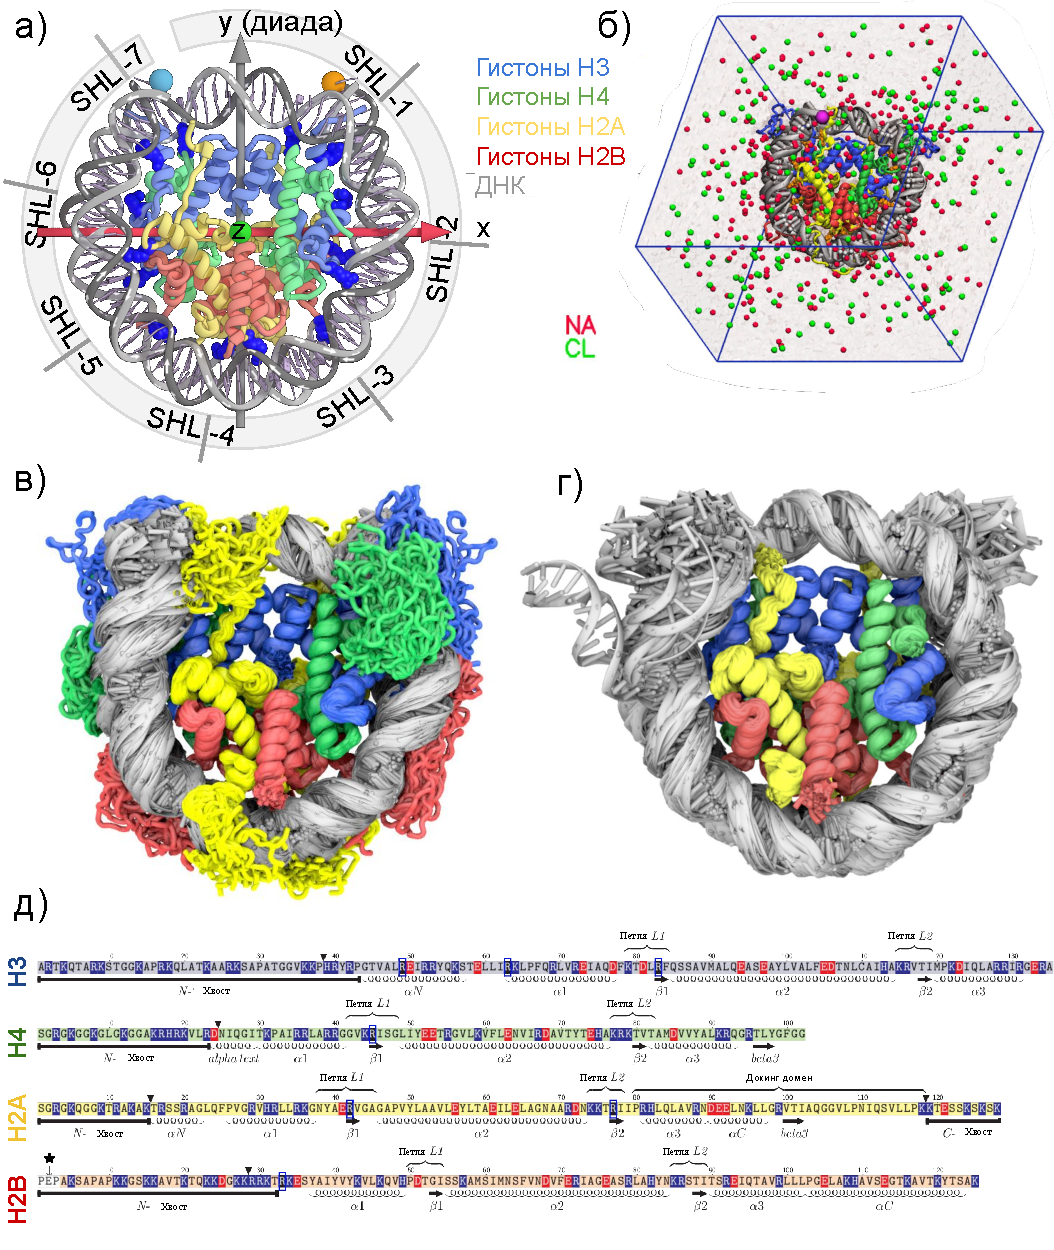
\includegraphics[width=0.95\textwidth]{images/p2/10ms/fig1.pdf}
    \caption[Системы нуклеосом моделируемые на временах более 10 мкс]{Системы нуклеосом моделируемые на временах более 10 мкс. а) Ключевые оси нуклеосомной системы отсчета. б) Вид моделируемой системы в ячейке с растворителем и ионами. c) Наложение кадров системы NCP$_{147} $каждые 100 нс. г) Наложение кадров NCP$^{nt}_{145}$ каждые 100 нс. д) Последовательность коровых гистонов и особенности их вторичной структуры ($ \alpha $ - спирали, $ \beta $ -листы, петли, гибкие хвосты гистонов). $ \blacktriangledown $ отмечает позиции обрезания хвостов в модели с усеченными хвостами; аргинины, боковые цепи которых вставлены малые бороздки ДНК отмечены синими рамками; синим отмечены - положительно заряженные остатки, красным - отрицательно заряженные остатки. $*$ отмечает PEP-конец H2B, который отсутствует в рекомбинантном варианте белка.}
    \label{fig:p2_3:f1}
\end{figure}

\begin{table}[p]
\caption{Список моделируемых систем}
\label{tbl:p2_3:systems}
\begin{threeparttable}
\begin{tabular}{lcp{8cm}c}
\hline
\textbf{Имя}& \textbf{PDB ID}\tnote{a} & \textbf{Описание}&\textbf{Время, мкс}\\ \hline\hline
NCP$_{147}$ & 1KX5 & 147 п.н. псевдосимметричной $\alpha$-сателлитной ДНК, гистоны полной длины в симметричном стартовом состоянии & 13.0  \\ \hline
NCP$^{fixed}_{147}$  & 1KX5 & Такая же как NCP$_{147}$, но C$\alpha$-атомы гистоновых фолдов ограничены в движении &  5.0  \\ \hline
NCP$^{nt}_{147}$ & 1KX5 & Такая же как NCP$_{147}$, но гистоновых хвосты обрезаны\tnote{b} &  10.0  \\ \hline
NCP$^{nt}_{146}$ & 1AOI & 146 п.н. $\alpha$-сателлитная ДНК, обрезанные гистоновые хвосты\tnote{b} & 7.0 \\ \hline
NCP$^{nt}_{145}$ & 3LZ0 & 145 п.н. 601-ой последовательности ДНК, обрезанные гистоновые хвосты\tnote{b} & 13.5  \\ \hline
\end{tabular}
\begin{tablenotes}
     \item[a] Иденификатор структуры, использованной для создания системы, из базы данных PDB.
     \item[b] Сайты обрезки хвостов определены на рис. \ref{fig:p2_3:f1}д.
   \end{tablenotes}
\end{threeparttable}
\end{table}


\subsubsection{Механизмы отворачивания и приворачивания ДНК}

Для анализа отворачивания ДНК от гистонового октамера нами был разработан подход определения количества отвернуты пар нуклеотидов ДНК для каждого кадра траектории. Для каждой пары нуклеотидов вычислялось ее ближайшее расстояние до какой-либо пары нуклеотидов кристаллической структуры. Количество отвернутых пар нуклеотидов с каждого конца определялось как максимальна длина сегмента ДНК от конца ДНК в котором расстояние для всех нуклеотидных пар от любых кристаллических положений было более 7 \AA. На основе данной меры были построены графики зависимости величины отворота ДНК от времени (Рис. \ref{fig:p2_3:f2_new}, Рис. \ref{fig:p2_3:f2}a,б и интерактивные материалы \url{http://intbio.github.io/nucl_MD_15mus/}).

Для систем без гистоновых хвостов ДНК сохраняла исходное привернутое положение в течение начального времени моделирования. Для разных расчетов и сторон нуклеосомы оно колебалось от 0.8 мкс до 4, 6 и более 7 мкс (см. Рис. \ref{fig:p2_3:f2_new}). Для системы с гистоновыми хвостами отворачивание началось на 4-ой микросекунде расчетов. Величина отворота ДНК составляла порядка 12-13 пар нуклеотидов, а в случае систем без хвостов иногда достигала 28 пар нуклеотидов. Рассмотрим в начале механизмы отворота ДНК в системе без хвостов. Анализ стабильных контактов гистонов и нуклеосом показывает, что конец ДНК в нуклеосомном коре формирует плотные контакты и удерживается взаимодействиями с аминокислотными остатками H3 гистона, в особенности H3Y41, H3R42, H3T45, которые находятся в области, которую мы назовем областью ``защелки'' концов ДНК \ref{fig:p2_3:f6}. Плотные взаимодействия в этой области удерживают конец ДНК в NCP. При отвороте ДНК данные взаимодействия нарушаются и ДНК переходит во флуктуирующее состояние, в котором величина отворота быстро меняется в наносекундном диапазоне (см. Рис. \ref{fig:p2_3:f2_new}, состояние \textbf{2}). В некоторых случаях плотные контакты застежки с ДНК восстанавливаются и система переходит в кристаллоподобное состояние (например в системе NCP$_{145}^{nt}$ на третьей наносекунде моделирования). Однако может произойти реконфигурация области защелки в гистоне H3 в состояние, не способное к плотному связыванию ДНК. Это приводит к тому, что флуктуационное состояние становится более долгоживущим и сопровождается также флуктуациями области H3 хвоста (см. Рис. \ref{fig:p2_3:f2_new}, состояние \textbf{2b}). Это флуктуационное состояние может разрешаться в кристаллоподобное состояние ДНК, когда остатки H3 смогут сформировать плотные контакты с флуктуирующим концом ДНК. Более детальный визуальный анализ взаимодействия гистона H3 с концом ДНК показал, что стабильное кристаллоподобное состояние ДНК возникает, когда ряд остатков входят в малую бороздку ДНК. В кристаллической структуре это H3R49, H3Y41, H3H39. Интересно, что в нашем моделировании в ряде систем (NCP$_{145}^{nt}$, NCP$_{145}^{nt}$) кристаллоподобное состояние ДНК также реализовывалось в состоянии, когда вместо H3H39 в малую бороздку заходил H3К40, который в кристалле взаимодействует с малой бороздкой другого супервитка (см. Рис. \ref{fig:p2_3:f2_new}, состояние \textbf{1b}). Дальнейшему откручиванию ДНК препятствовал стабильный сайт связывания с гистонов H2A в районе позиции -59, с которой контактируют остатки H2AK75, H2AT76, H2AR77 из L2 петли. На 14-ой микросекунде в системе NCP$_{145}^{nt}$ наблюдался дальнейший отворот до уровне 26-28 отвернутых пар оснований с диссоциацией контактов данного сайта(см. Рис. \ref{fig:p2_3:f2_new}, состояние \textbf{3}). Данный факт требует дальнейшего исследования. Масштаб флуктуаций ДНК в системе без хвостов представлен на рисунках \ref{fig:p2_3:f1}в,г. Важной особенностью является то, что ДНК откручивается не только в плоскости нуклеосомного диска, но и имеет компонент смещения вдоль суперспиральной оси нуклеосомы. Более подробно взаимоотношение смещения конца ДНК вдоль оси Х и Z представлено на рисунке \ref{fig:p2_3:f1}ж. Существенной корреляции между смещениями не наблюдается, однако очевидно, что при больших параметрах отворота наблюдается в основном состояния с некоторым компонентом смещения вдоль оси суперспирали в направление противоположное от внутреннего супервитка ДНК. Данный факт можно объяснить стерическим и электростатическим отталкиванием витков ДНК.

В отличие от систем без гистоновых хвостов, система с хвостами ведет себя несколько по другому (Рис. \ref{fig:p2_3:f1}б,д,е). Мы также наблюдали откручивание до 12-14 пар оснований с конца ДНК, однако существуют существенные отличия. Во-первых, величина отклонения открученных пар нуклеотидов от их кристаллического пути была меньше из-зи того, что гистоновые хвосты оказывали удерживающее воздействие на конформацию ДНК и ее возможность отклонятся в различных направлениях. Во-вторых, флуктуации ДНК между состояниями с различной степенью откручивания были менее выражены по амплитуде, опять же из-за воздействия гистоновых хвостов, главным образом N-хвоста гистона H3 и С-конца гистона H2A. Наличие гистоновых хвостов приводит к расщеплению динамического состояния отворота-приворота 12 концевых нуклеотидов, наблюдаемого в системе без хвостов, на ряд подсостояний определяемых конформацией гистоновых хвостов. Рисунок \ref{fig:p2_3:f1}и иллюстрирует среднее время приворота ДНК из состояний с заданной величиной отворота. Из рисунка видно, что наличие гистоновых хвостов серьезным образом влияет на увеличение времени приворота ДНК. Для величины отворота в 10 пн время возрастает с 20-40 нс до $\sim$100 нс. Гистоновые хвосты также существенным образом влияют на механизм отворачивания ДНК. Мы наблюдали, что область ``защелки'' H3 гистона также, как и в случае системы без хвостов, теряет контакты с сегментом ДНК вблизи входа-выхода, однако, потери этих контактов способствует внедрение N-конца гистона H3 между супервитками ДНК. Хвост H3 с одной стороны образует дополнительные контакты с ДНК, но с другой стороны способствует замещению стабильных контактов с область H3-``защелки''. Этот же эффект приводит к тому, что в отличие от системы без гистоновых хвостов, хвост H3 может препятствовать быстрому привороту ДНК из отвернутого положения в привернутое.

Более подробно динамика взаимодействия ДНК с H3-``защелкой'' и взаимодействие хвостов гистонов с концами нуклеосомной ДНК представлена на рисунке \ref{fig:p2_3:f3}.

\begin{figure} [H]
    \centering
    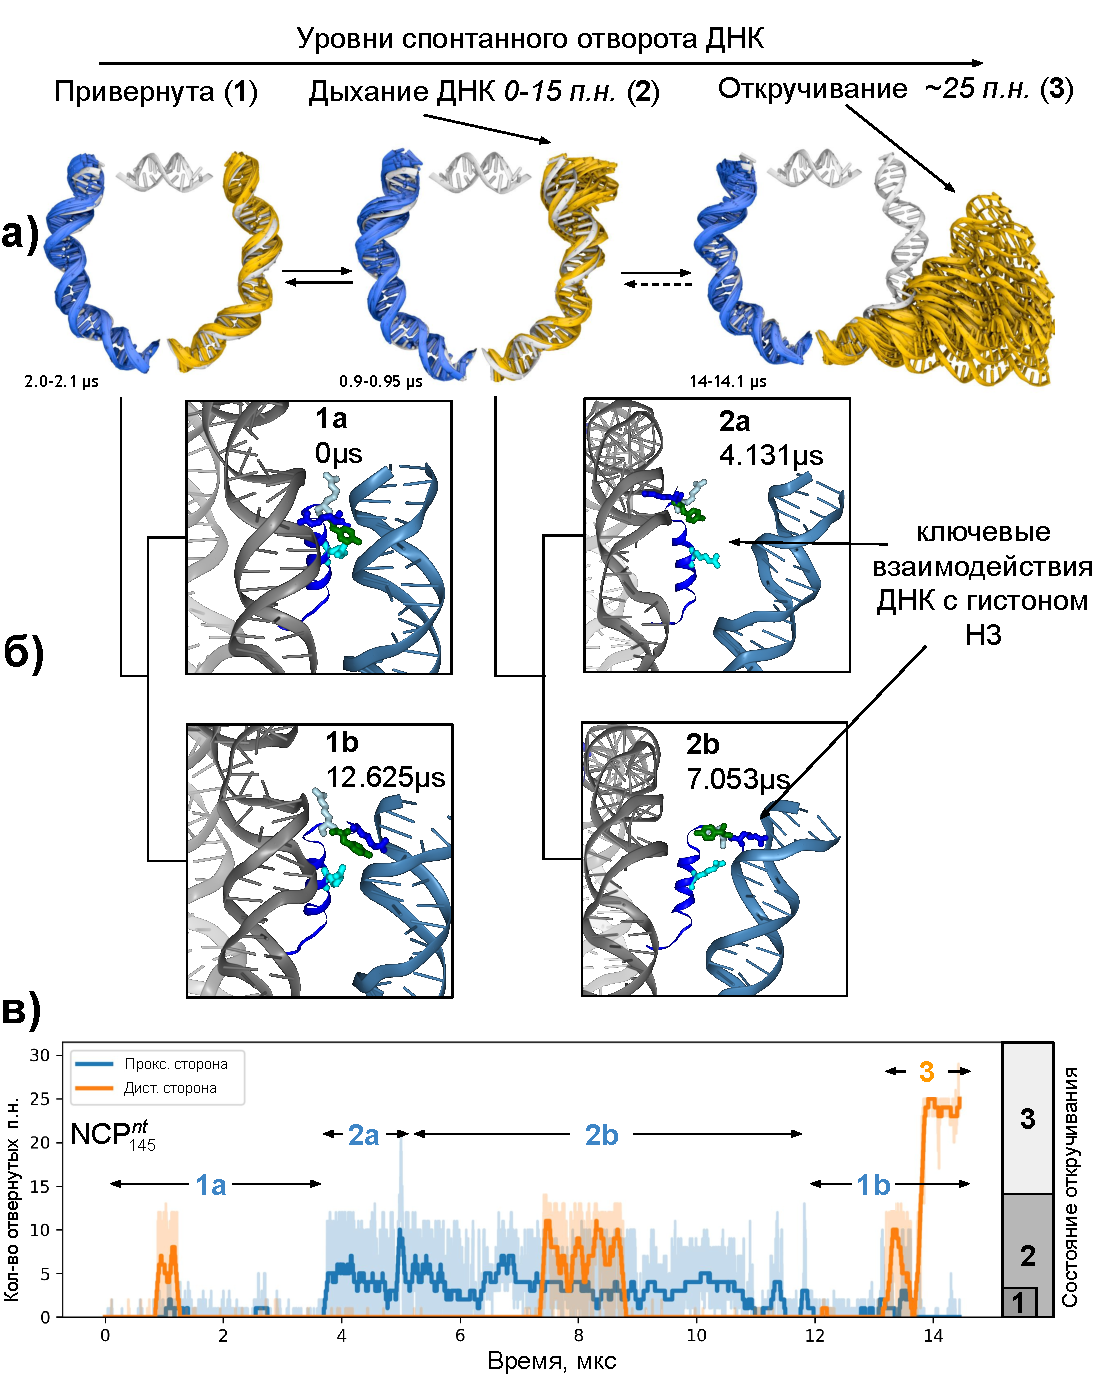
\includegraphics[width=\textwidth]{images/p2/10ms/fig2_new.pdf}
    \caption[Динамика отворота ДНК в нуклеосоме с укороченными гистоновыми хвостами]{Динамика отворота ДНК в нуклеосоме с укороченными гистоновыми хвостами (наблюдаемая в системе NCP$^{nt}_{145}$). Количество пар нуклеотидов отвернутых от октамера гистонов как функция времени моделирования представлена снизу. Критерий отворота ДНК  --  смещение центра пары оснований более, чем на 7 \AA{} от положений оснований в исходной структуре. Наблюдается три состояния \textbf{1-3} (изображены сверху). Для состояний \textbf{1} и \textbf{2} наблюдаются подсостояния, связанные с реориентацией H3 $\alpha$N спирали и области H3-``застежки'' (средний ряд изображений).}
    \label{fig:p2_3:f2_new}
\end{figure}



\begin{figure} [H]
    \centering
    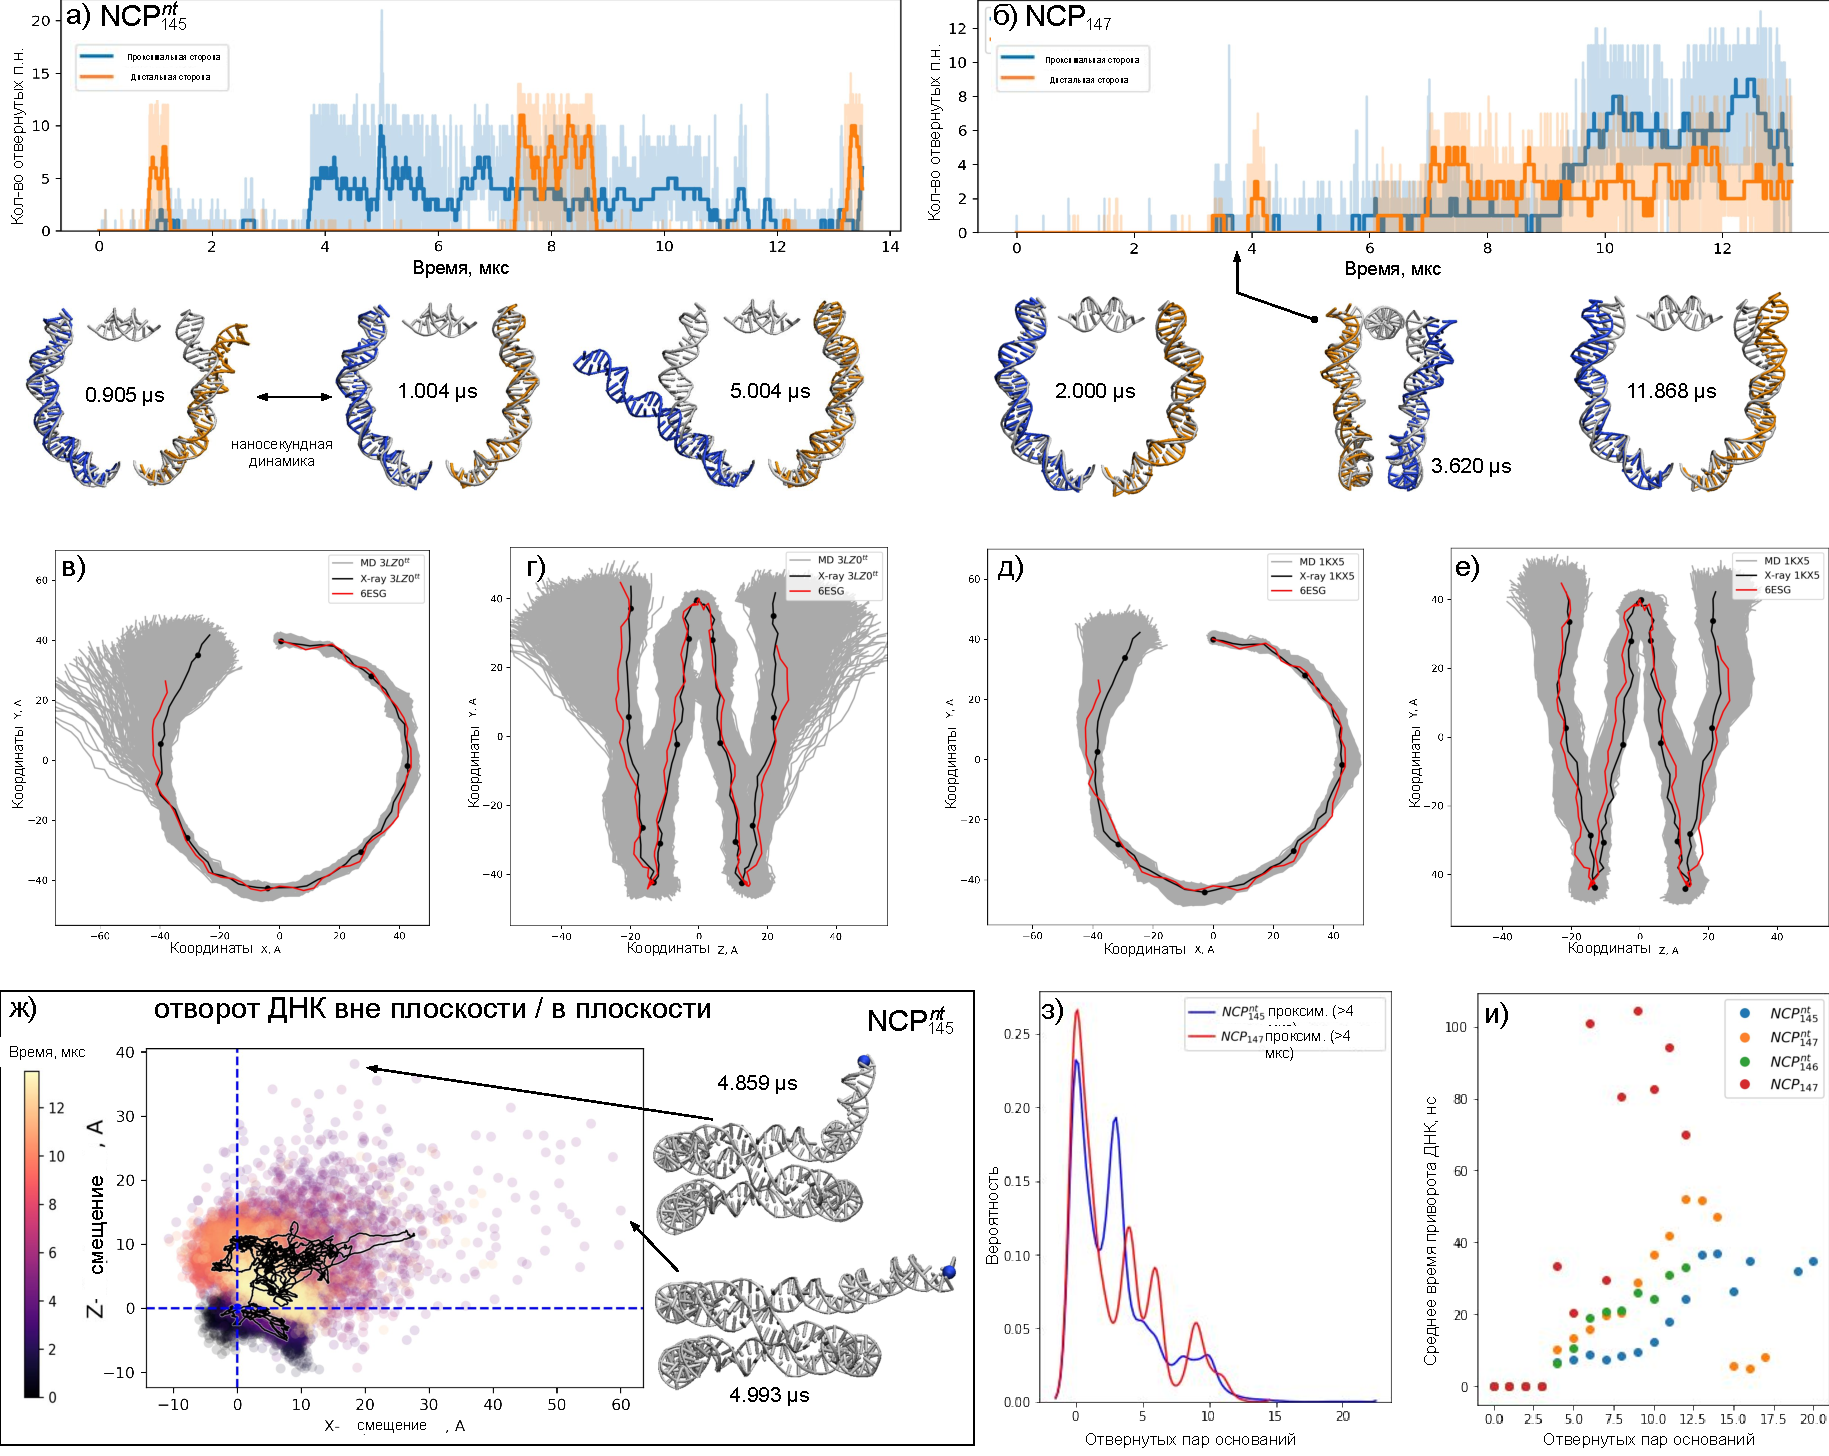
\includegraphics[width=\textwidth]{images/p2/10ms/fig2.pdf}
    \caption[Сравнение характеристик отворота ДНК в нуклеосомах с и без гистоновых хвостов]{Сравнение характеристик отворота ДНК в нуклеосомах с и без гистоновых хвостов. а)-б) отворот ДНК с течением времени для NCP$^{nt}_{145}$ и NCP$_{147}$, определенных как смещение центра пары оснований более, чем на 7 \AA{} от положений оснований в исходной структуре. в-е) Проекции центров пар оснований ДНК на различные плоскости СКН. ж) Смещение проксимального конца ДНК в ходе МД. з) Распределений вероятности отворота ДНК. и) Среднее время приворота ДНК из состояния с определенным отворотом.}
    \label{fig:p2_3:f2}
\end{figure}





\begin{figure}[H]
    \centering
    %DNA ends are coupled to the inner DNA dyre via a  histone H3 residues.
    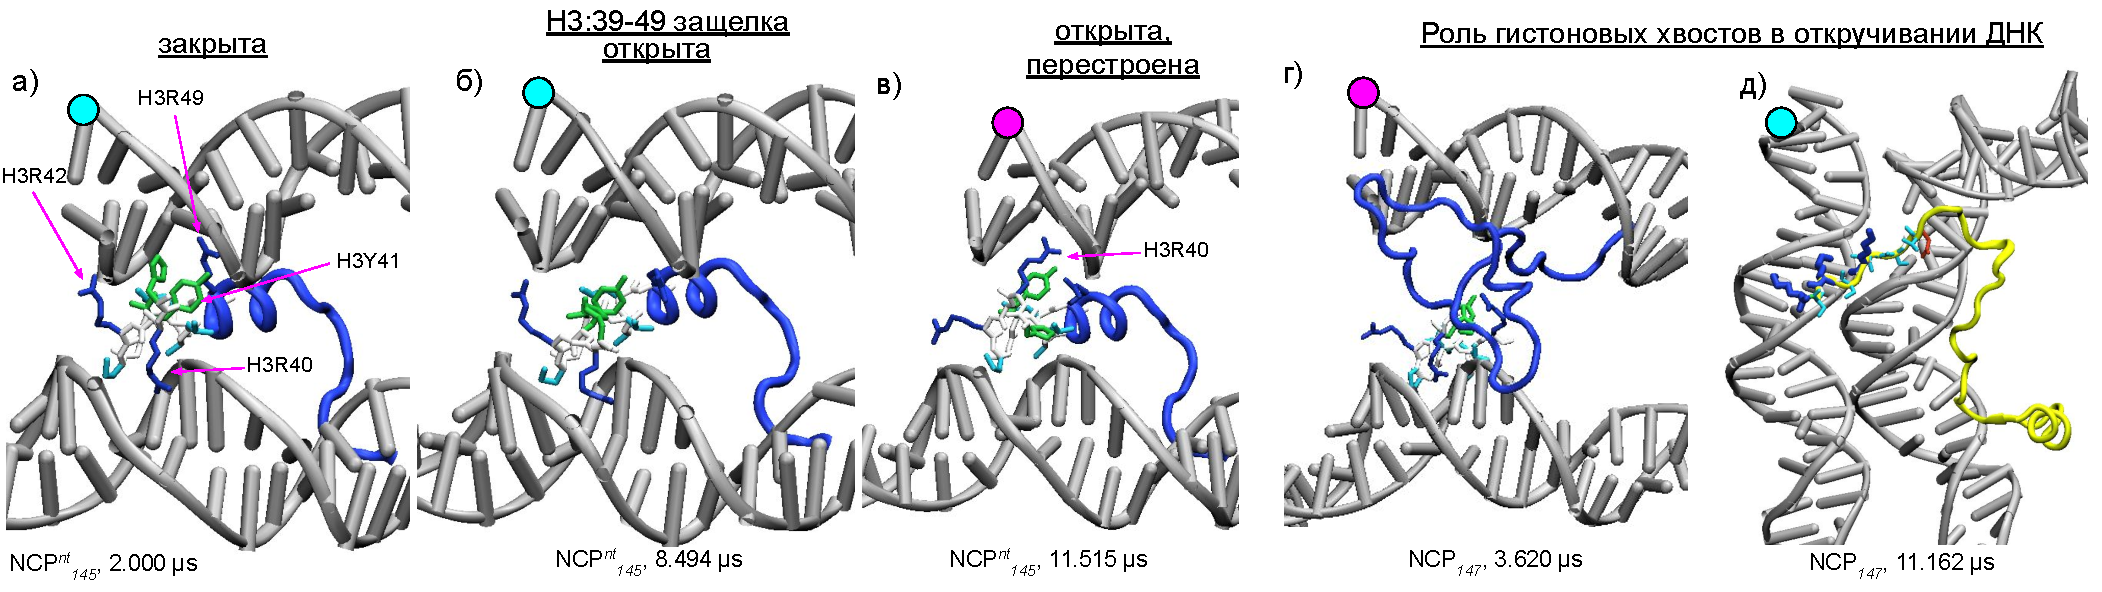
\includegraphics[width=\textwidth]{images/p2/10ms/fig3.pdf}
    \caption[Динамика ``защелки'' концов ДНК фрагментом гистона H3]{Динамика ``защелки'' концов ДНК фрагментом гистона H3}
    \label{fig:p2_3:f3}
\end{figure}



Каковым может быть функциональное значение отворачивания ДНК концов от гистонового кора? С одной стороны предполагается, что отворачивание ДНК необходимо для связывания различных факторов транскрипции \cite{li_rapid_2005}. В нашем моделировании для системы с гистоновыми хвостами ДНК не достигала такой степени отворота. Однако плотное взаимодействие хвостов с ДНК скорее всего распространится и на более существенные степени отворота ДНК. Таким образом, мы предполагаем, что важным фактором для определения доступности ДНК для транскрипционных факторов будет не только отворот ДНК, но и взаимодействия ДНК с гистоновыми хвостами. Другим возможным эффектом отворачивания ДНК является влияние изменение конформации нуклеосомальной ДНК на возможную укладку нуклеосом на супрануклеосомном уровне. Для оценки данных эффектов мы провели моделирование, в котором генерировали фибриллы из 10 нуклеосом, соединяя прямыми отрезками линкерной ДНК длиной 17 п.н. случайно выбранные  кадры из траекторий. Таким образом, можно было получить ансамбль конформаций нуклеосомных фибрилл и оценить распределение длин между концами фибрилл (Рис. \ref{fig:p2_3:f4}). По сравнению с фибриллами построенными на основе кристаллической структуры, фибриллы построенные с учетом флуктуаций концов коровой ДНК демонстрировали в среднем расстояние между концами на 10-15 нм больше. Ширина самого распределения составляла около 20 \AA. Таким образом, можно сделать вывод о том, что динамика концов ДНК, во-первых, ``разрыхляет'' супрануклеосомную структуру хроматина, а, во-вторых, обеспечивает достаточную конформационную гибкость фибриллы в пределах тепловых колебаний ($\sim$kT). 



\begin{figure}[H]
    \centering
    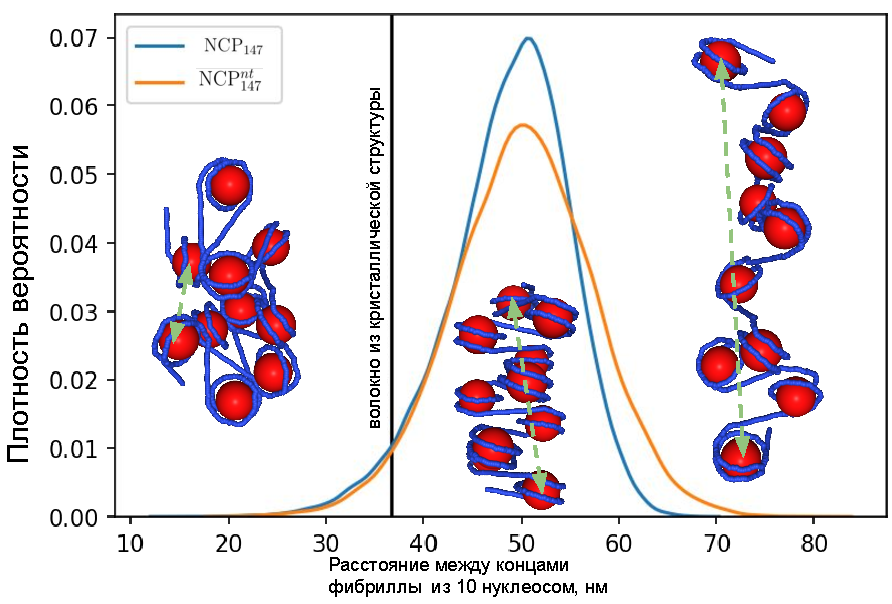
\includegraphics[width=\textwidth]{images/p2/10ms/fig4.pdf}
    \caption[Влияние динамики ДНК на структуру хроматиновых фибрилл]{Влияние динамики ДНК на структуру хроматиновых фибрилл}
    \label{fig:p2_3:f4}
\end{figure}


\subsubsection{Динамика кручения ДНК в нуклеосоме}

Интересным фактом в ходе моделирования явилось наблюдение релаксации дефекта кручения ДНК внутри нуклеосомного кора в системе NCP$_{147}^{nt}$. Дефект кручения ДНК в этой системе, основанной на 601-ой последовательности ДНК, располагается в районе SHL $\pm$5. По сравнению с нуклеосомами на основе альфа-сателлитной ДНК, ДНК в районе этого положения растянута на 1 нуклеотид, при этом совершает то же самое количество оборотов (см. рисунок \ref{fig:p2_3:f5}г). В ходе моделирования мы наблюдали резкий перескок регистра ДНК из кристаллоподобного состояния (Рис. \ref{fig:p2_3:f5}б) в состояние, где нуклеотиды начиная с нуклеотида номер -54 сместились в сторону диады нуклеосомы. Рисунок  \ref{fig:p2_3:f5}д иллюстрирует то, что данный сдвиг регистра ДНК далее произошел для всего конца ДНК, начиная приблизительно с нуклеотида -50. Таким образом около 20 нуклеотидов с проксимального конца ДНК испытали вращательное движение внутри нуклеосомного кора. Любопытным является изучение деталей данного механизма. Рассмотрение динамики отворачивание ДНК свидетельствует о том, что релаксация дефекта кручения произошла в области, которая не была затронута отворотом ДНК (Рис. \ref{fig:p2_3:f2}а). В то же время нельзя исключить, что отворот концов ДНК способствовал релаксации дефекта и его распространению вдоль ДНК. С точки зрения стальных контактов в системе NCP$_{145}^{nt}$ в районе SHL -6 в течение первой микросекунды моделирования наблюдался стабильный контакт нижней цепи ДНК в положении -58 с H2AT76 и верхней цепи ДНК в положении -54 с H2BS56. При анализе 10 микросекунды моделирования на предмет стабильных контактов между нуклеотидами и аминокислотами оказалось, что первый контакт остался неизменным, а второй контакт сместился на нуклеотид за номером -55. Таким образом, релаксация данного дефекта кручения была в некотором роде асимметрична. В большей степени наблюдалось сдвиг регистра контактов для верхней цепи ДНК. Интересным фактом является то, что как недавно было показано в структурных работах по изучению механизмов работ ремоделеров нуклеосом семейства ISWI и SWI/SNF, именно, верхняя цепь ДНК изменяет свое положение на нуклеосомном коре в первую очередь при связывании АТФ субъединицы ремоделера \cite{li_mechanism_2019}.

Еще одним интересным фактом сопровождающим релаксацию дефекта кручения ДНК в районе SHL -5 является деформация в этот момент спирали $\alpha2$ H2A гистона с отгибом ее С-конца в сторону центра нуклеосомного кора. С-конец данной спирали связан с сайтом связывания ДНК в районе SHL -5.5 и, вероятно, участвует в ослаблении контактов ДНК с гистоновым кором, которое помогает релаксации дефекта кручения.


\begin{figure}[H]
    \centering
    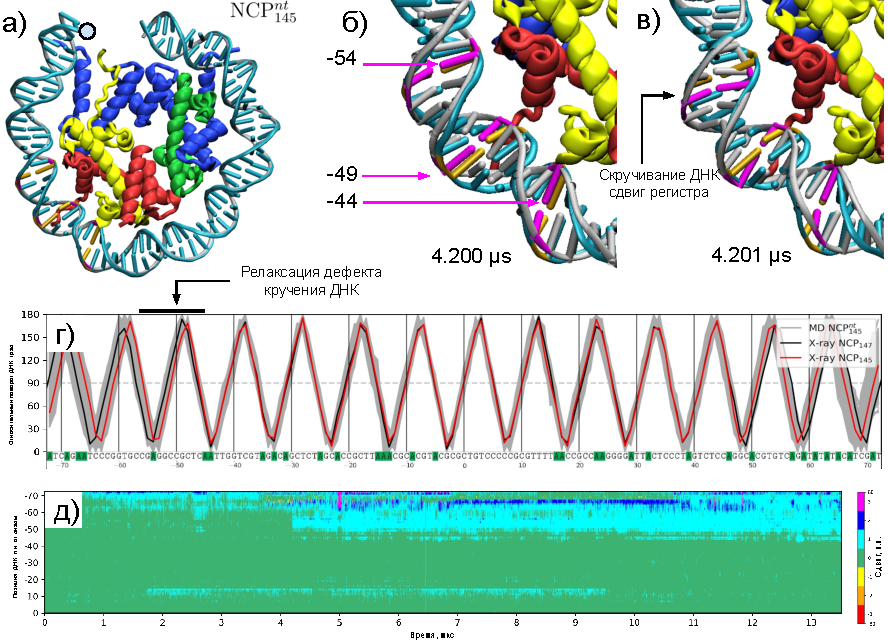
\includegraphics[width=\textwidth]{images/p2/10ms/fig5.pdf}
    \caption[Динамика кручения ДНК в нуклеосоме]{Динамика кручения ДНК в нуклеосоме. а) Структура проксимального супервитка нуклеосомы в начальный момент. Кристаллическая форма ДНК изображена голубым цветом, серым цветом ДНК в ходе МД моделирования. Оранжевым цветом отмечены пары нуклеотидов, которые участвуют изменяют положение на нуклеосоме. б) Кадр траектории до прокручивания ДНК. в) Кадр траектории после прокручивания ДНК. г) График параметра относительного кручения (relative twist) ДНК на нуклеосоме. д) Иллюстрация сдвига в положении нуклеотидов для верхней цепи ДНК относительно положения в кристаллической структуре.}
    \label{fig:p2_3:f5}
\end{figure}



\subsubsection{Динамика контактов ДНК-белок в нуклеосоме}

Наличие траекторий молекулярной динамики позволяет достаточно точно описать взаимодействия гистонов с ДНК на уровне контактов отдельных атомов, аминокислот, нуклеотидов. Причем в отличие от анализа кристаллических структуру имеется возможность оценить устойчивость и динамическую подвижность тех или иных контактов. Нами был проведен анализ стабильных контактов между аминокислотными остатками гистонов и нуклеотидами ДНК. Для изначального анализа была выбрана система NCP$_{147}$ в течение первой микросекунды моделирования, когда отворота ДНК не наблюдалась. Также поскольку система является псевдосимметричной мы учитывали только те контакты, которые присутствовали с обеих сторон нуклеосомы. Результат анализа приведена на рисунке \ref{fig:p2_3:f6}. Данные график иллюстрирует все основные особенности связывания ДНК с гистонами. Обратим внимание на две особенности, которые по нашему мнению имеют функциональное значение. Количество контактов, которые образует верхняя цепь ДНК значительно меньше, контактов которые образует нижняя цепь ДНК. Предполагаем, что это как раз может иметь значение при передвижении нуклеосом вдоль ДНК АТФ-зависимыми ремоделерами, которые как было показано недавно в первую очередь вытягивают и деформируют верхнюю цепь ДНК. Второй интересный момент связан с наличием области H3 гистона, которую мы называем ``защелкой'', которая взаимодействует как с концом коровой ДНК, так и с областью вблизи диады - около положения -9. Отметим, что вблизи положения -9 в геномных исследованиях по позиционированию нуклеосом наблюдается необычный сигнал - там чаще встречаются нуклеотиды A/T, хотя по общему правилу нуклеосомы предпочитают в области изгиба ДНК в сторону большой бороздки нуклеотиды G/C \cite{davey_does_2013}. Данные факт может отчасти объясняться плотным взаимодействием H3R40 внутри малой бороздки ДНК с электроотрицательным группами A/T оснований.


\begin{figure} [H]
    \centering
    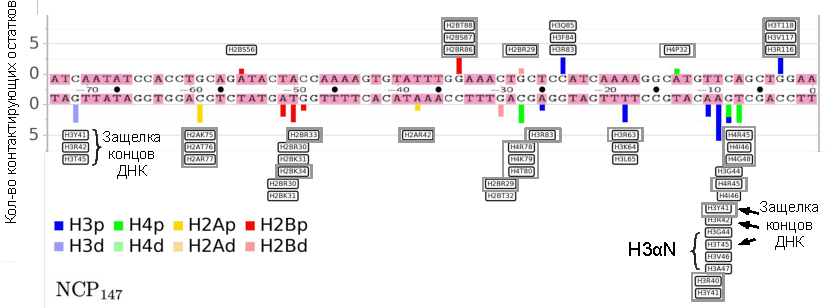
\includegraphics[width=\textwidth]{images/p2/10ms/fig6.pdf}
    \caption[Стабильные контакты ДНК-гистоны в нуклеосоме]{Стабильные контакты ДНК-гистоны в нуклеосоме. Отмечены контакты между нуклеотидами и аминокислотными остатками, присутствующие в 90\% кадров в системе NCP$_{147}$ в течение первой микросекунды моделирования с обоих симметричных сторон нуклеосомы. В рамках отмечены контакты, которые сохраняются с обоих сторон нуклеосомы в течение всей МД траектории.}
    \label{fig:p2_3:f6}
\end{figure}

\subsubsection{Пластичность гистонового октамера}

Как было описано во введении весьма актуальной темой научных исследований на данный момент является изучение пластичности октамера гистонов. Для исследования данного вопроса нами были построены проекции координат атомов $\alpha 2$-спиралей гистонов на плоскость нуклеосомного диска (Рис. \ref{fig:p2_3:f7}. Видно, что спирали испытывают флуктуации в пределах от нескольких до 5-6\AA. Особенно выделяются флуктуации концов C-концов спиралей гистона H2A. Недавно методами крио-ЭМ был разрешен ряд деформированных структур нуклеосомного кора, в частности структура нуклеосомы сжатая вдоль диадной оси на несколько процентов. RMSD кадров  МД траектории относительно данной структуры (Рис. \ref{fig:p2_3:f7}в) показывает, что данная структура зачастую отличается от кадров траектории не более, чем начальная структура самой траектории. Таким образом, можно сделать вывод, что наблюдаемые в эксперименте деформированные состояния нуклеосом находятся, по крайней мере, в рамках отличий, которые мы видим между кадрами траектории на масштабе мультимикросекундного моделирования.

В ряде работ было показано, что дисульфидные сшивки внутри димеров гистонов приводят к изменению функционирования нуклеосом. В частности H3L82C-H4V81C уменьшает термическую диффузию нуклеосом по ДНК и влияет на работу ремоделера SNF2h \cite{bilokapic_histone_2018,bilokapic_structural_2018,sinha_distortion_2017}. Расстояние между С-$\alpha$ атомами данные остатков изображена на рисунке \ref{fig:p2_3:f7}г. Оно колеблется в пределах от 6,1-8,5\AA. Длина дисульфидной связи составляет около 2,05\AA, расстояние между С-$\alpha$-атомом и атомом серы в стандартной конформации цистеина составляет 2,81\AA и не меняется при вращении торсионных углов. Таким образом максимальное расстояния между С-$\alpha$-атомами у остатков цистеина, связанных дисульфидной связью, составляет 7,67\AA. Следуя данным расчетам, видим, что дисульфидная сшивка будет препятствовать некоторым конформациям, наблюдаемым в динамике.

Для того, чтобы дополнительно изучить влияние пластичности октамера на динамику ДНК, мы провели расчеты, в которых $\alpha 2$-спирали гистонов были зафиксированы. Анализ флуктуационной динамики ДНК показал (см. рисунок \ref{fig:p2_3:f7}е), что у системы с фиксированными $\alpha$-спиралями подвижность ДНК была снижена на всем ее протяжении. Данные эффект требует дальнейшего изучения, однако можно предположить, что уменьшение подвижности ДНК отрицательно сказывается на возможности ремоделирования и скольжения нуклеосом.



\begin{figure} [H]
    \centering
    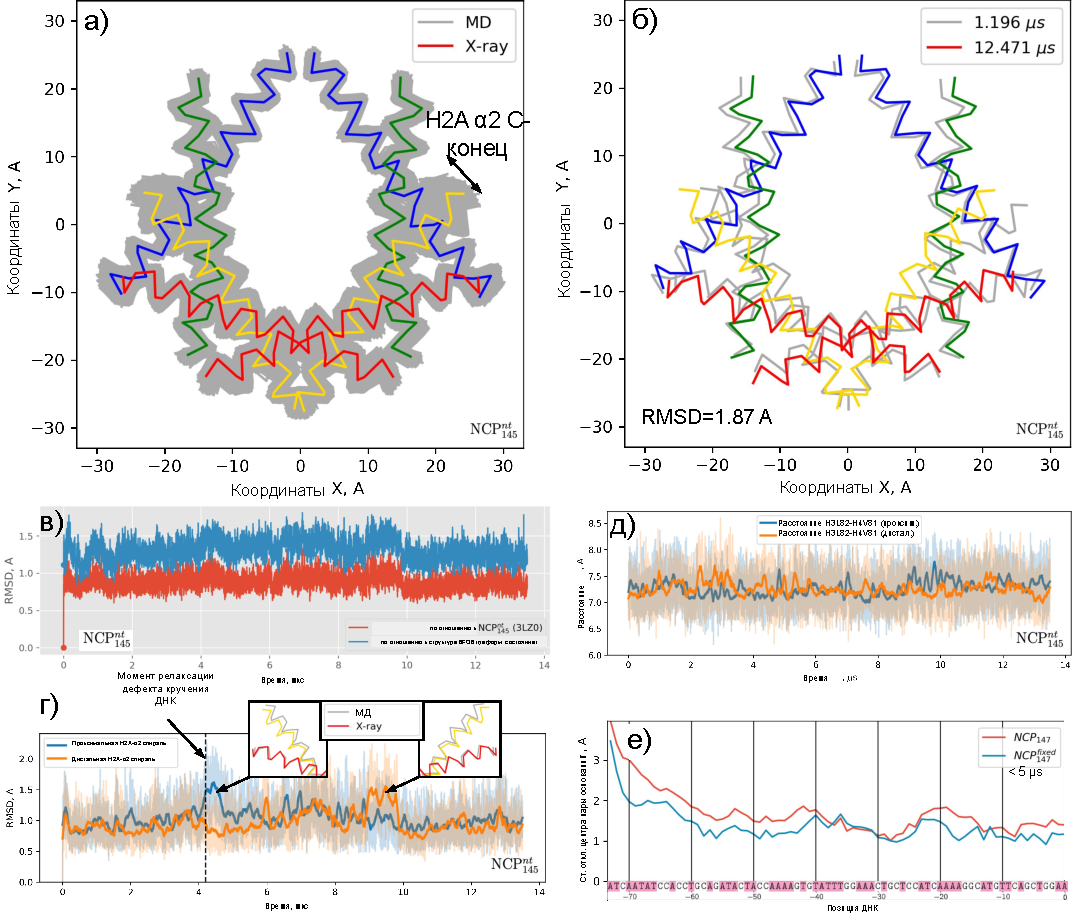
\includegraphics[width=\textwidth]{images/p2/10ms/fig7.pdf}
    \caption[Пластичность гистонового октамера]{Пластичность гистонового октамера. а) Наложение проекций координат С$\alpha$-атомов $\alpha 2$-спиралей гистонов в плоскости нуклеосомального диска из кадров МД траектории. б) Аналогичные проекции координат С$\alpha$-атомов для двух кадров с максимально различным RMSD. в) RMSD $\alpha 2$-спиралей гистонов в ходе МД относительно исходной структуры и структуры 6FQ6, полученной крио-ЭМ, с деформированной конформацией ядра нуклеосомы. г) Эволюция RMSD спирали $\alpha 2$ гистона H2A. д) Расстояние между остатками, которые подвергаются дисульфидным сшивкам в ряде экспериментов. e) Сравнение флуктуаций пар оснований ДНК в системах с закрепленными и незакрепленными $\alpha 2$-спиралями гистонов.}
    \label{fig:p2_3:f7}
\end{figure}

\subsubsection{Аллостерическая связь откручивания ДНК и конформации ДНК около диады}

Область ``застежки'' гистона H3 взаимодействует одновременно с двумя супервитками ДНК. Это наблюдение известно достаточно давно. Например, Horn et al. в своих экспериментах наблюдали, что SIN мутация гистона H4R25C взаимодействующая в положении SHL $\pm$0.5 приводит к ухудшению возможности компактизации нуклеосомальных фибрилл. Они предположили, что одним из возможных механизмов является дестабилизации концов нуклеосомальной ДНК в виду коммуникации области SHL $\pm$0.5 с областями SHL $\pm$6.5 посредством H3 $\alpha$N-спирали. Однако, Flaus et al. предположили, что этот эффект может объясняться увеличением мобильности нуклеосом и их смещению относительно исходных позиций \cite{flaus_sin_2004}. Тем не менее, нам было интересно рассмотреть в нашем моделировании возможные эффекты коммуникации областей SHL $\pm$0.5 и SHL $\pm$6.5. На рисунке \ref{fig:p2_3:f9} приведен сравнительных анализ откручивания ДНК и деформации ДНК в различных положениях от времени для системы NCP$_{147}$. Любопытным является факт, что вслед за откручиванием ДНК, зачастую область ``защелки'' гистона H3 теряет свои контакты не только с концом ДНК, но и с областью нижнего супервитка.
Такой случай изображен на панели \ref{fig:p2_3:f9}в. Потеря контактов с нижним супервитком ДНК в свою очередь ведет к деформации ДНК в этой области и к ее усиленным флуктуациям. Можно предположить, что наличие флуктуация в нижнем супервитке будет способствовать прохождению через нуклеосому дефектов скручивания ДНК.

В результате анализа приведенного в данном разделе нами выдвигается предположение о наличие динамической (аллостерической) связи между откручиванием ДНК и скольжению нуклеосом вдоль ДНК по механизму продвижения дефектов кручения. Откручивание концов коровой ДНК, во-первых, помогает образованию и прохождению дефектов скручивания вблизи концов ДНК, а, во-вторых, способствует дестабилизации ДНК в районе диады, что также, вероятно, помогает прохождению дефектов скручивания далее через нуклеосомную ДНК.



\begin{figure} [H]
    \centering
    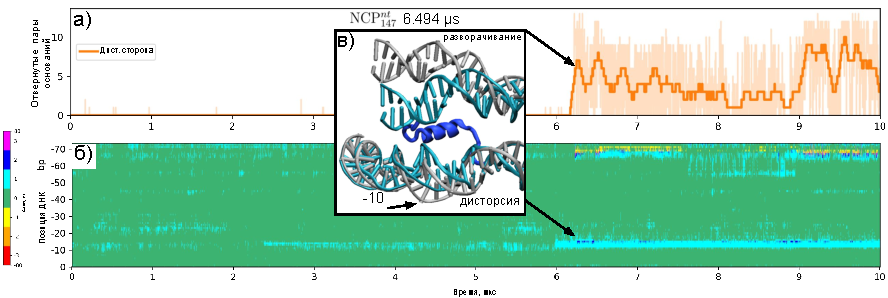
\includegraphics[width=\textwidth]{images/p2/10ms/fig9.pdf}
    \caption[Аллостерическая связь откручивания ДНК и конформации ДНК около диады]{Аллостерическая связь откручивания ДНК и конформации ДНК около диады. а) График откручивание ДНК от времени в ходе МД моделирования. б) График смещения нуклеотидов относительно кристаллической структуры.}
    \label{fig:p2_3:f9}
\end{figure}





\subsection{Благодарности}

Работа данного раздела поддержана грантами Российского научного фонда № 18-74-10006 (атомистическое моделирование нуклеосом и разработка и анализ траекторий нуклеосом), грантами Российского фонда фундаментальных исследований № 20-34-70039 (моделирование структуры супрануклеосомальных фибрилл) и № 19-34-51053 (метода анализа взаимодействий белков и нуклеиновых кислот). Исследования проводились на оборудовании коллективных исследовательских установок вычислительных ресурсов высокопроизводительных вычислений МГУ им. М.В. Ломоносова.